%%%%%%% PAQUETES Y CONFIGURACIONES %%%%%%% INICIO
\documentclass[11pt,letter]{article}

% Idioma y codificación
\usepackage[utf8]{inputenc}
\usepackage[spanish]{babel}

% Diseño de página
\usepackage[left=2.54cm,right=2.54cm,top=2.54cm,bottom=2.54cm]{geometry}
\usepackage{setspace}
\usepackage{float}

% Tipografía y matemáticas
\usepackage{amsmath}
\usepackage{pifont}
\usepackage{amsfonts}


% Colores (debe ir antes de tcolorbox y pgfplots)
\usepackage[table,xcdraw]{xcolor}

% Gráficos y figuras
\usepackage{graphicx}
\usepackage{longtable}
\usepackage{pgfplots}
\pgfplotsset{compat=1.18}

% Tablas y cajas
\usepackage{booktabs}
\usepackage[most]{tcolorbox}
\usepackage{mdframed}

% Algoritmos y código
\usepackage[linesnumbered,ruled,vlined]{algorithm2e}
\usepackage{listings}

% Referencias y notas
\usepackage{nameref}
\usepackage{natbib}
\usepackage{endnotes}

% Hipervínculos (último siempre que sea posible)
\usepackage{hyperref}

%Para dar ancho a tabla
\usepackage{tabularx}

% Centrado de tablas
\usepackage{array}
\newcolumntype{C}[1]{>{\centering\arraybackslash}m{#1}} % Centrado horizontal y vertical


%%%%%%% PAQUETES Y CONFIGURACIONES %%%%%%% FIN


\begin{document}
\onehalfspacing

%%%%%%% PORTADA %%%%%%% INICIO
\begin{titlepage}
\centering

\includegraphics[width=0.15\textwidth]{resources/universidad-del-valle.png}\par\vspace{1cm}
{\scshape\LARGE Universidad del Valle \par}
{\scshape\Large Facultad de Ingeniería \par}
{\scshape\Large Escuela de Ingeniería de Sistemas y Computación \par}
\vspace{2cm}

{\Large \textbf{Minimizando el Extremismo Presente en
 una Población (MinExt)}}\\

\vspace{2cm}
    {\large \textbf{Anderson Johan Alban Angulo - 202310006}}\\
    {\large \textbf{Andrés Felipe Asprilla Urrutia - 202224101 }}\\
    {\large \textbf{Andrés Mauricio Ortiz Bermúdez - 202110330}}\\
    {\large \textbf{Carlos Mauricio Tovar Parra - 201741699}}\\
\vspace{2cm}

    \Large\textbf{Profesor}\par
    {\large \textbf{Jesús Alexander Aranda Bueno Ph.D.}}\\
\vspace{1.4cm}
    \Large\textbf{Curso}\par
    {\large \textbf{Análisis y Diseño de Algoritmos II (750020C)}}\\
\vspace{1cm}
{\large {26 de julio de 2025}\par}
\end{titlepage}
%%%%%%% PORTADA %%%%%%% FIN

%%%%%%% INDICE %%%%%%% INICIO
\tableofcontents
%%%%%%% INDICE %%%%%%% FIN
\newpage

%%%%%%% INTRODUCCIÓN %%%%%%% INICIO
\section{Introducción}

El fenómeno del extremismo ha cobrado especial relevancia en las sociedades actuales, caracterizándose por una polarización creciente de las opiniones en grupos claramente diferenciados. Este proyecto aborda el problema de la minimización del extremismo (MinExt), el cual busca reducir el nivel total de extremismo dentro de una población, tomando como base un conjunto inicial de opiniones diversas. Para esto, se plantea la implementación de un modelo de optimización que permita decidir cuáles personas cambiarán sus opiniones iniciales, con el objetivo de alcanzar la menor cantidad posible de extremismo, considerando costos limitados en términos económicos y logísticos.

El presente trabajo se desarrolla mediante técnicas avanzadas de programación entera mixta y optimización combinatoria, utilizando el método Branch and Bound y herramientas de modelamiento como MiniZinc. El proyecto también incluye el diseño de una interfaz gráfica que permite a un usuario final interactuar de manera intuitiva con el modelo desarrollado.

%%%%%%% INTRODUCCIÓN %%%%%%% FIN
\newpage


\newpage
%%%%%%% FUERZA BRUTA %%%%%%% INICIO
\section{El modelo: Descripción y Justificación de su Adecuación}

El modelo implementado para resolver el problema \texttt{MinExt} se fundamenta en los siguientes componentes:

\subsection{Parámetros de Entrada}
\begin{itemize}
  \item $n$: Número total de personas en la población.
  \item $m$: Número de posibles opiniones.
  \item $p_i$: Número inicial de personas con opinión $i$.
  \item $\mathit{ext}_i$: Valor de extremismo de la opinión $i$.
  \item $c_{i,j}$: Costo de mover personas de opinión $i$ a opinión $j$.
  \item $c^e_i$: Costo extra por mover personas hacia opiniones inicialmente desocupadas.
  \item $c_t$: Costo total máximo permitido.
  \item $\max M$: Número máximo permitido de movimientos totales.
\end{itemize}

\subsection{Variables de Decisión}
\begin{description}
    \item[Variable] $x_{i,j}$
    \item[Definici\'on] Representa el n\'umero de personas que cambiaron de la opini\'on $i$ a la opini\'on $j$.
    \item[Dominio] $i, j \in [1, m]$, donde $x_{i,j} \in \mathbb{N}$.
    \item[Prop\'osito] Esta variable permite cuantificar y analizar las transiciones entre diferentes opiniones, proporcionando una base para evaluar la din\'amica de cambio de opini\'on en el modelo y para aplicar estrategias de moderaci\'on si es necesario.
\end{description}


\subsection{Restricciones}
\begin{itemize}
    \item \textbf{Costo Máximo (Lineal):}
    Esta restricción limita el costo total de todos los movimientos a un presupuesto máximo \texttt{ct}. Se clasifica como \textbf{lineal} porque la variable \texttt{costo} es de tipo \texttt{float} (continua).
    $$
    \text{costo} \le \text{ct}
    $$

    \item \textbf{Límite de Movimientos (Lineal y Entera):}
    Asegura que el total de movimientos realizados no supere el límite \texttt{maxM}. Es una restricción \textbf{lineal y entera} porque la variable \texttt{movimientosTotales} es de tipo \texttt{int} y se compara con una constante entera.
    $$
    \text{movimientosTotales} \le \text{maxM}
    $$

    \item \textbf{Conservación de la Población de Origen (Lineal y Entera):}
    Para cada opinión $i$, esta restricción clave impide que se muevan más personas de las que existen inicialmente en esa opinión ($p_i$). Es \textbf{lineal y entera}, ya que opera sobre sumas de las variables enteras $x_{i,j}$.
    $$
    \forall i \in [1, m]: \sum_{j=1}^{m} x_{i,j} \le p_i
    $$

    \item \textbf{Prohibición de Movimientos Nulos (Lineal y Entera):}
    Impide las transiciones de una opinión a sí misma, fijando la diagonal de la matriz $x$ a cero. Es una restricción simple \textbf{lineal y entera}.
    $$
    \forall i \in [1, m]: x_{i,i} = 0
    $$

    \item \textbf{Límite de Población Total (Lineal y Entera):}
    Garantiza que el número total de personas movidas no exceda la población total $n$. Es \textbf{lineal y entera} porque \texttt{personaOpinion} es \texttt{int}.
    $$
    \text{personaOpinion} \le n
    $$

    \item \textbf{Movimientos entre Extremismos Iguales (Lineal y Entera):}
    Prohíbe mover personas entre dos opiniones distintas si estas comparten el mismo valor de extremismo. Es una restricción \textbf{lineal y entera} que reduce el espacio de búsqueda.
    $$
    \forall i, j \in [1, m] \text{ donde } \text{ext}_i = \text{ext}_j \implies x_{i,j} = 0
    $$

    \item \textbf{No Negatividad (De Cota):}
    Son restricciones de cota que aseguran que las variables no tomen valores negativos. Son un tipo fundamental de restricción lineal y entera.
    \begin{itemize}
        \item $\text{costo} \ge 0$
        \item $\text{movimientosTotales} \ge 0$
        \item $\forall i, j \in [1, m]: x_{i,j} \ge 0$
    \end{itemize}
\end{itemize}
\subsection{Función Objetivo y Propósito del Modelo}

\subsubsection{Fórmula del Objetivo}
El objetivo principal del modelo es \textbf{minimizar} el extremismo total de la población en su estado final. La función objetivo se define como:

$$
\text{minimizar } \sum_{i=1}^{m} \text{nueva\_p}_i \cdot \text{ext}_i
$$

Donde $\text{nueva\_p}_i$ es una variable que representa la población final en la opinión $i$ después de aplicar todos los movimientos $x_{i,j}$.

\subsubsection{Explicación y Justificación}

\paragraph{Explicación:}
La función objetivo calcula una métrica de \textbf{extremismo agregado} para toda la población. Esto se logra a través de una suma ponderada: para cada opinión posible, se multiplica su extremismo (el parámetro $ext_i$) por el número de personas que finalmente pertenecen a esa opinión (la variable $nueva\_p_i$). De esta manera, las opiniones con valores altos de extremismo y una gran cantidad de adherentes contribuyen más al valor total de la función.

\paragraph{Justificación:}
El propósito fundamental del modelo es encontrar la estrategia de moderación más efectiva que se ajuste a las restricciones de recursos (como el costo $ct$ y el número de movimientos $maxM$). Al establecer la minimización del extremismo total como el objetivo, el modelo no se limita a realizar movimientos al azar. En cambio, el solver está instruido para encontrar la combinación de movimientos $(x_{i,j})$ que deliberadamente desplace a la población de opiniones más extremas a otras menos extremas, resultando en el menor valor posible de la función objetivo.

\section{Datos Relevantes de la Implementación}

Para llevar a la práctica la solución del problema \texttt{MinExt}, se desarrolló una aplicación web que facilita la interacción del usuario con el modelo de optimización, desde la carga de datos hasta la visualización de los resultados. La arquitectura de la solución se basa en una clara separación entre el cliente y el servidor.

\paragraph{Desarrollo del Backend:} El servidor de la aplicación fue desarrollado en \textbf{Python} utilizando el micro-framework \textbf{Flask}, el cual se encarga de gestionar las rutas y la lógica de negocio. El backend es responsable de recibir los archivos de instancia \texttt{.txt} cargados por el usuario, validarlos y procesarlos. Una vez que los datos son parseados, el servidor genera dinámicamente un archivo de datos en formato \texttt{.dzn}, que es el formato requerido por MiniZinc para definir los parámetros de una instancia específica del problema. Posteriormente, invoca al motor de \textbf{MiniZinc} a través de un subproceso del sistema, especificando el uso del solver \textbf{Coin-BC (COIN-OR Branch and Cut)}. Una vez que el solver finaliza, el backend captura la salida, la procesa para extraer las métricas clave y la envía al frontend en un formato JSON estructurado.

\paragraph{Desarrollo del Frontend:} La interfaz de usuario fue construida con \textbf{HTML}, \textbf{CSS} y \textbf{JavaScript}. Para la manipulación dinámica del contenido y la comunicación asíncrona con el servidor se utilizó la biblioteca \textbf{jQuery}, que permite realizar solicitudes AJAX para enviar el archivo de instancia y recibir los resultados sin necesidad de recargar la página. La presentación visual de los datos se enriquece mediante el uso de \textbf{Chart.js}, que se utiliza para mostrar tanto la distribución inicial de la población como la distribución final obtenida tras la optimización. El diseño y la maquetación se apoyan en el framework de CSS \textbf{TailwindCSS}.

\paragraph{Flujo de Interacción:} El proceso completo es transparente para el usuario final. Comienza cuando el usuario selecciona un archivo de instancia en la interfaz. El frontend envía este archivo al servidor Flask. El servidor lo procesa, ejecuta el modelo de optimización y, tras obtener una respuesta del solver, la devuelve al cliente. Finalmente, el frontend interpreta los datos recibidos y actualiza la vista dinámicamente, mostrando tablas con resúmenes numéricos, la matriz de movimientos y gráficos comparativos que permiten un análisis visual e inmediato de la efectividad de la solución encontrada.

\paragraph{Descripción del modelo en MiniZinc.}
La implementación del problema se materializó en un modelo declarativo utilizando el lenguaje MiniZinc. El diseño del modelo inicia con la definición de un conjunto de \textbf{parámetros de entrada} que caracterizan cualquier instancia del problema, como la población, los costos y los niveles de extremismo. El núcleo del problema reside en la \textbf{variable de decisión} principal, una matriz \texttt{x} que representa el flujo de personas entre cada par de opiniones. Para mejorar la legibilidad y la modularidad, se utilizan \textbf{variables} que encapsulan cálculos complejos, como el costo total (incluyendo una lógica condicional para los cargos extra), el total de movimientos y la distribución final de la población. El comportamiento del sistema está regido por un conjunto de \textbf{restricciones} explícitas que definen el espacio de soluciones factibles, asegurando el cumplimiento de los límites de recursos, la conservación de la población y las reglas lógicas del negocio. Finalmente, el modelo establece una \textbf{función objetivo} clara: minimizar el extremismo total en la distribución final de opiniones, instruyendo así al solver para que encuentre la solución óptima entre todas las configuraciones posibles.


\begin{tcolorbox}[colback=green!5!white, colframe=green!50!black, title=Factibilidad y Escalabilidad de la Solución]
El tiempo necesario para encontrar una solución válida depende directamente del tamaño de la población (n) y del número de posibles opiniones (m), ya que estos parámetros influyen en la complejidad y el costo del modelo. Cuanto mayor sean n y m, mayor será el costo y el tiempo de procesamiento. Además, el número de recursos disponibles también impacta en la rapidez con la que el modelo puede generar una solución. Para asegurar que la solución sea tanto precisa como factible, el modelo toma en cuenta restricciones clave, incluyendo limitaciones en el número de movimientos y los costos adicionales asociados con los cambios de opiniones no representadas inicialmente. Esto permite respetar los límites de recursos y garantiza que las soluciones propuestas sean realistas y alcanzables.
        \end{tcolorbox}
\section{Análisis Branch and Bound}

El árbol de búsqueda generado por el solver Gecode/Gist proporciona un mapa visual del proceso de razonamiento seguido para encontrar la solución óptima. A través del método \textit{Branch and Bound}, el solver explora sistemáticamente el espacio de soluciones, podando ramas que no pueden conducir a un resultado mejor que el ya encontrado. A continuación, se detalla el recorrido del árbol paso a paso.

\subsubsection*{Instancia de Prueba Utilizada}
A continuación se presenta la instancia en formato \texttt{.dzn} que fue resuelta para generar el árbol de búsqueda analizado. Los parámetros de costo (\texttt{ct}) y movimientos (\texttt{maxM}) fueron ajustados para forzar al solver a tomar decisiones de ramificación estratégicas.

\begin{itemize}
    \item $n = 20$
    \item $m = 5$
    \item $p_i = [8, 6, 4, 2, 0]$
    \item $\mathit{ext}_i = [1.0, 0.8, 0.5, 0.2, 0.1]$
    \item $c_{i,j} = \bordermatrix{
              & \mathbf{1} & \mathbf{2} & \mathbf{3} & \mathbf{4} & \mathbf{5} \cr
        \mathbf{1} & 0   & 8.0 & 5.0 & 3.0 & 1.0 \cr
        \mathbf{2} & 10.0& 0   & 4.0 & 2.0 & 3.0 \cr
        \mathbf{3} & 15.0& 12.0& 0   & 1.0 & 2.0 \cr
        \mathbf{4} & 18.0& 15.0& 12.0& 0   & 1.0 \cr
        \mathbf{5} & 25.0& 22.0& 20.0& 18.0& 0 \cr
    }$
    \item $c^e_j = [10.0, 10.0, 10.0, 10.0, 40.0]$
    \item $c_t = 6.0$
    \item $\max M = 7$
\end{itemize}

\subsubsection*{Visualización del Árbol de Búsqueda}
La ejecución de la instancia anterior con el solver Gecode/Gist generó el siguiente árbol de búsqueda, que sirve como base para el análisis del recorrido.
\begin{figure}[H]
            \centering
            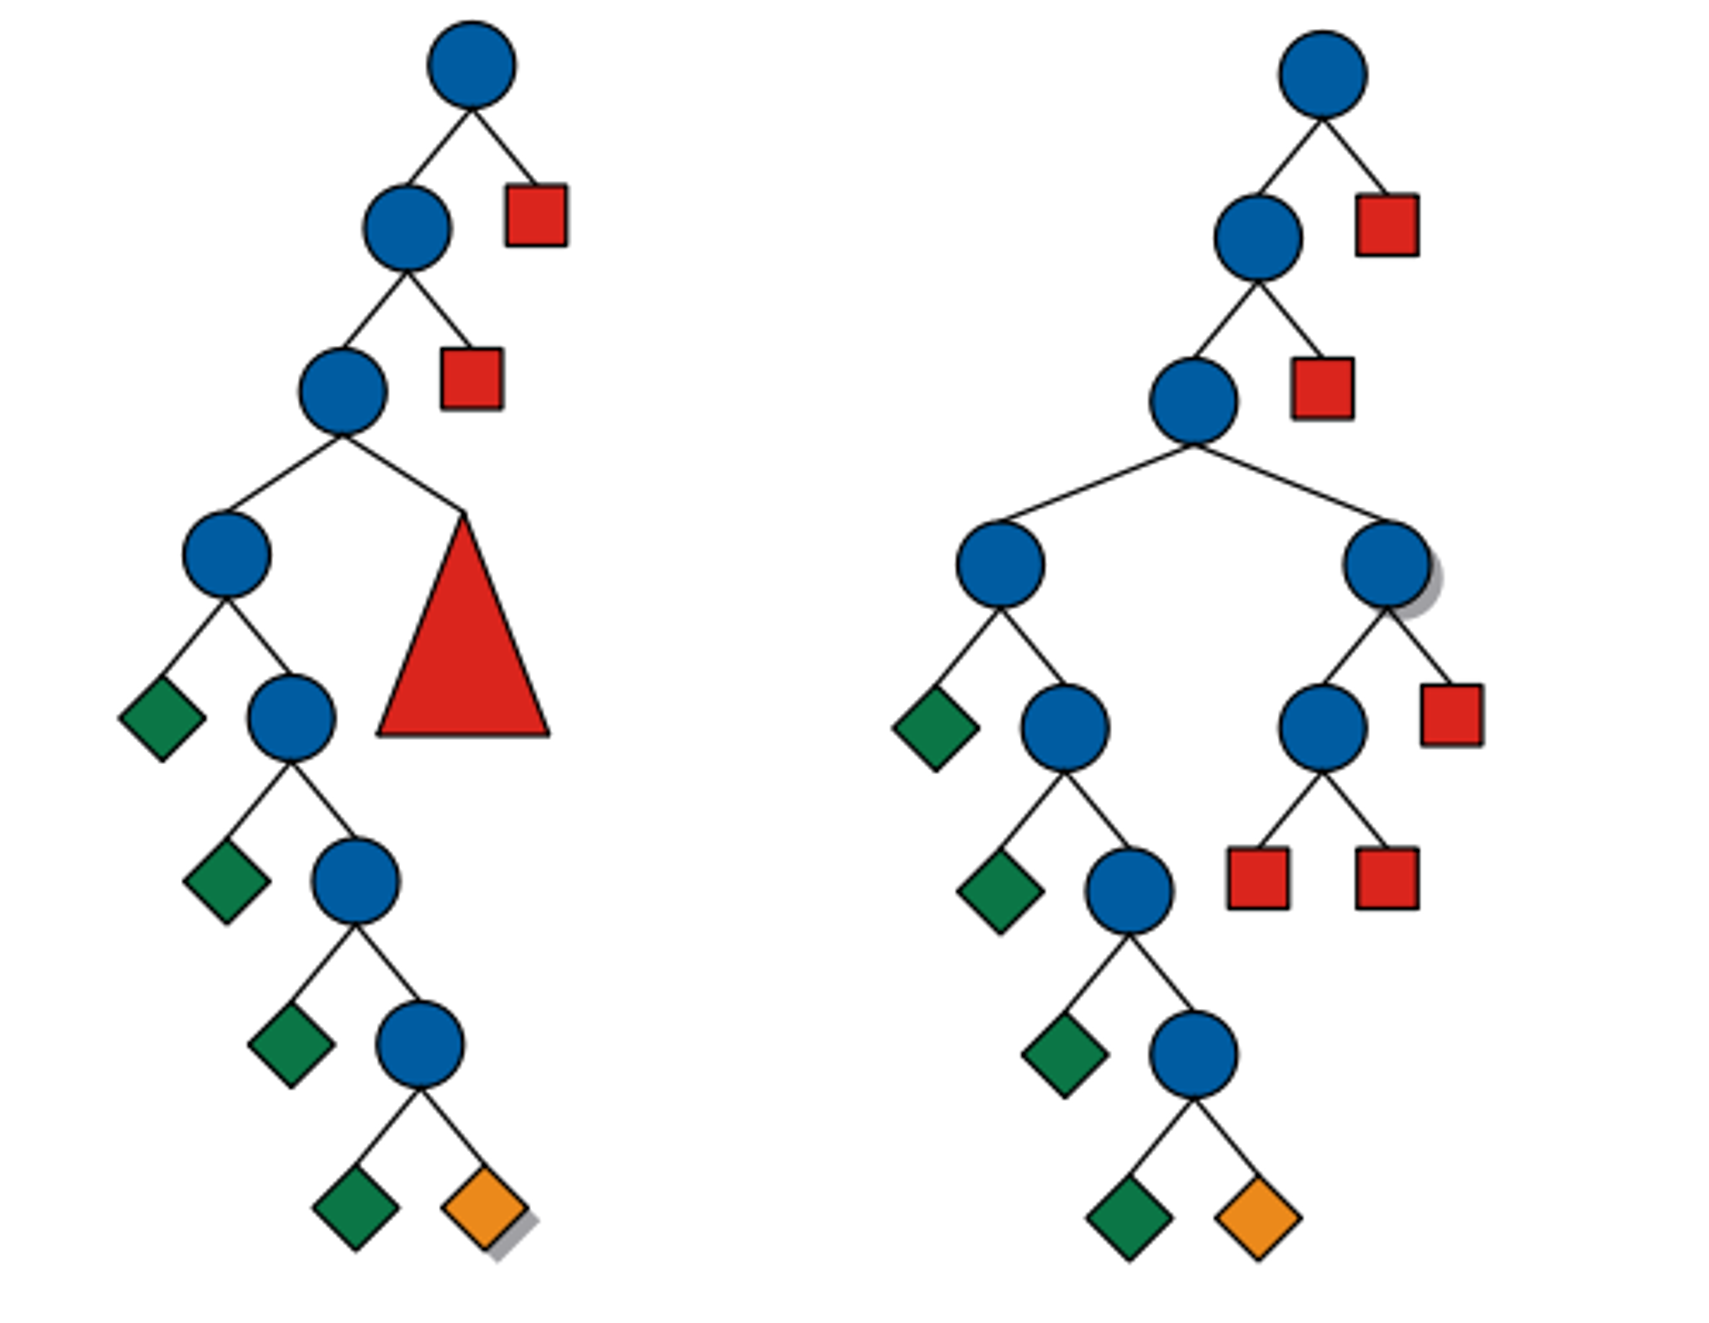
\includegraphics[width=0.4\textwidth]{resources/branchandbound.png}
            \caption{Expansión del Arbol Branch and Bound.}
        \end{figure}

\paragraph{Paso 1 - El Punto de Partida (Nodo Raíz):}
La búsqueda se inicia en el nodo raíz (\textbf{el círculo azul superior}). En este estado inicial, el solver solo ha procesado los parámetros de entrada y las restricciones. Las variables de decisión aún no tienen valores fijos, sino que se representan por sus dominios iniciales, que son amplios y reflejan todas las posibilidades teóricas. Por ejemplo, el costo potencial se encuentra en un rango inicial de \texttt{[0..19.4]}, y las variables de movimiento (\texttt{x}) permiten múltiples transiciones. El objetivo en este punto es comenzar a tomar decisiones para acotar este vasto espacio de búsqueda.

\paragraph{Paso 2 - Exploración Inicial y Poda por Infactibilidad:}
El solver desciende por el árbol y comienza a tomar las primeras decisiones. En los niveles superiores, se encuentra rápidamente con nodos de fallo (\textbf{los cuadrados rojos}). Estos nodos representan estados en los que se ha violado una o más restricciones de manera irreparable. Por ejemplo, al intentar un movimiento, el costo acumulado puede haber excedido el límite \texttt{ct} o el número de movimientos el límite \texttt{maxM}. Al detectar esta infactibilidad, el solver aplica la técnica de \textit{poda (pruning)}, descartando por completo estas ramas y evitando así una exploración innecesaria. El solver retrocede (backtracking) y continúa por el único camino que, hasta el momento, sigue siendo viable.

\paragraph{Paso 3 - El Punto de Ramificación (El Triángulo Rojo):}
A medida que desciende, el solver llega a un punto crítico, representado por el \textbf{triángulo rojo}. Este nodo es un \textbf{punto de ramificación (branching point)}. Aparece porque la simple propagación de restricciones ya no es suficiente para que el solver deduzca el siguiente paso. Se enfrenta a un dilema y debe tomar una decisión estratégica sobre una variable que aún no está fija. Para resolverlo, crea dos o más ramas nuevas, una para cada posible decisión. En este caso, el análisis de la expansión del triángulo revela lo siguiente:
\begin{itemize}
    \item \textbf{Exploración de la Rama Derecha:} El solver elige explorar una de las nuevas ramas. Este camino resulta ser infructuoso. Al seguirlo, los nodos subsiguientes (\textbf{los cuadrados rojos dentro de la expansión del triángulo}) rápidamente violan una restricción. En este caso, aunque el costo se mantenía dentro del rango, es probable que se haya superado el número máximo de movimientos permitidos (\texttt{maxM}). El solver poda esta sub-rama por completo.
    \item \textbf{Exploración de la Rama Izquierda:} Tras el fallo anterior, el solver retrocede y explora la otra alternativa creada en el punto de ramificación. Este camino resulta ser prometedor y es el que el solver continuará explorando para buscar la solución óptima.
\end{itemize}

\paragraph{Paso 4 - Búsqueda de Soluciones y Mejora de la Cota:}
Continuando por el camino viable, el solver encuentra sus primeras soluciones completas y factibles, representadas por los \textbf{rombos verdes}. La primera de estas soluciones establece la \textbf{cota superior inicial (upper bound)} para la función objetivo (el \textit{récord a batir} de extremismo). Cada vez que se encuentra una nueva solución factible con un valor de extremismo inferior al récord actual, esta nueva solución se convierte en la mejor encontrada hasta ahora y la cota superior se actualiza. Esta cota es fundamental para el algoritmo, ya que le permite podar cualquier otra rama que, según sus cálculos, no tenga el potencial de generar una solución mejor que la que ya posee.

\paragraph{Paso 5 - Convergencia a la Solución Óptima:}
Finalmente, tras haber explorado o podado todas las ramas del árbol, el solver llega al \textbf{rombo naranja}. Este nodo representa la \textbf{solución óptima final}. En este punto, todas las variables de decisión tienen un valor específico. Para este problema, la solución óptima consistió en mover 4 personas de la opinión 3 a la 4, con un costo total de 4.8 y una distribución final de la población de \texttt{[8, 6, 0, 6, 0]}. El solver puede garantizar que esta es la mejor solución posible porque todas las demás alternativas han sido sistemáticamente evaluadas y descartadas, ya sea por ser infactibles o por conducir a soluciones de peor calidad que la óptima encontrada.

\section{Pruebas}

\subsection{Rendimiento del equipo}
Las pruebas fueron ejecutadas en un equipo con sistema operativo Windows 11 Pro, equipado con un procesador Intel(R) Core(TM) i7-9750H CPU @ 2.60GHz, con 6 núcleos físicos y 12 hilos lógicos, y 64 GB de memoria RAM. Para la resolución de las instancias se utilizó MiniZinc versión 2.9.3 (build 1832600886) junto con el solver COIN-BC 2.10.12/1.17.10. Este entorno computacional permitió llevar a cabo simulaciones de alta demanda, haciendo posible procesar casos complejos con grandes cantidades de personas, opiniones y restricciones.
\begin{figure}[H]
    \centering
    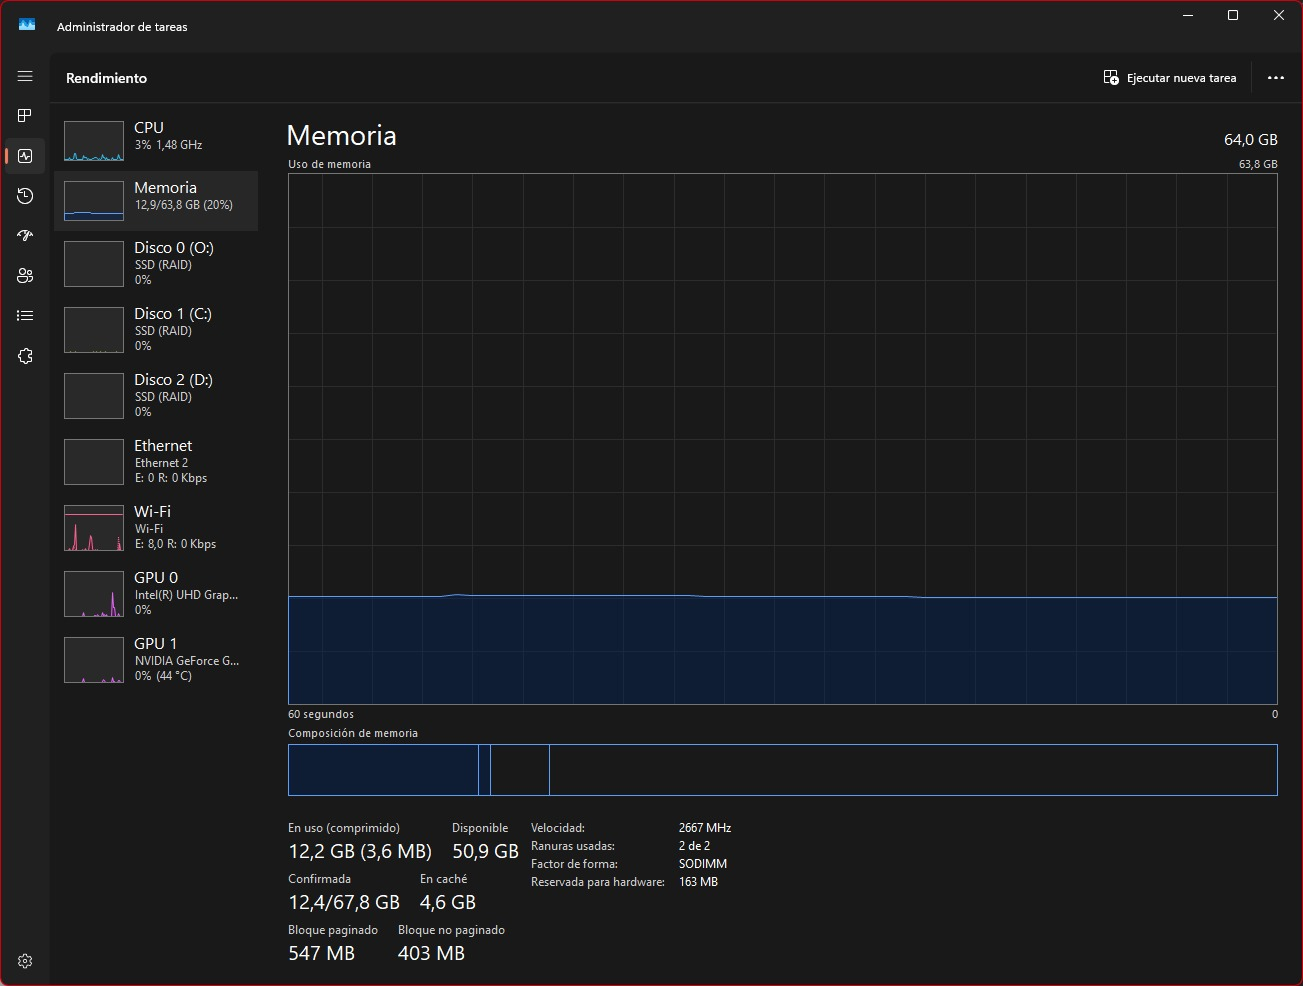
\includegraphics[width=0.7\textwidth]{resources/rendimientodelequipo.jpg}
    \caption{Rendimiento del equipo en el que se realizaron las pruebas}
\end{figure}


\subsection{Resultados obtenidos con las intancias de la batería de pruebas}

\begin{table}[H]
    \centering
    \small
    \resizebox{\textwidth}{!}{
    \begin{tabular}{|l|c|c|c|c|c|c|c|c|c|c|}
    \hline
    \textbf{Prueba} & \textbf{Personas} & \textbf{Opiniones} & \textbf{Costo Máximo} & \textbf{Mov. Máx.} & \textbf{Tiempo} & \textbf{Ext. Inicial} & \textbf{Ext. Final} & \textbf{Costo Total} & \textbf{Mov. Totales} & \textbf{\% Reducción} \\
    \hline
    Prueba1.txt & 10 & 5 & 75.01 & 9 & 0.17 & 6.145 & 3.846 & 22.74 & 9 & \textbf{37.4\%} \\
    Prueba2.txt & 10 & 5 & 24.14 & 4 & 0.19 & 7.409 & 4.582 & 8.35 & 4 & \textbf{38.2\%} \\
    Prueba3.txt & 10 & 5 & 81.78 & 22 & 0.19 & 2.905 & 0.261 & 72.53 & 14 & \textbf{91.0\%} \\
    Prueba4.txt & 10 & 5 & 96.95 & 25 & 0.16 & 3.844 & 1.06 & 19.65 & 11 & \textbf{72.4\%} \\
    Prueba5.txt & 10 & 5 & 128.25 & 1 & 0.18 & 5.369 & 4.448 & 4.12 & 1 & \textbf{17.1\%} \\
    Prueba6.txt & 15 & 5 & 60.84 & 10 & 0.18 & 12.123 & 9.583 & 29.05 & 10 & \textbf{21.0\%} \\
    Prueba7.txt & 15 & 5 & 141.96 & 25 & 0.17 & 5.275 & 0.829 & 76.64 & 25 & \textbf{84.3\%} \\
    Prueba8.txt & 20 & 5 & 112.21 & 27 & 0.2 & 8.367 & 3.541 & 38.99 & 27 & \textbf{57.7\%} \\
    Prueba9.txt & 20 & 5 & 87.46 & 9 & 0.17 & 8.645 & 3.654 & 33.3 & 9 & \textbf{57.7\%} \\
    Prueba10.txt & 20 & 5 & 17.35 & 32 & 0.18 & 13.303 & 10.353 & 16.79 & 18 & \textbf{22.2\%} \\
    Prueba11.txt & 40 & 10 & 151.21 & 58 & 0.19 & 15.22 & 2.12 & 130.0 & 58 & \textbf{86.1\%} \\
    Prueba12.txt & 40 & 10 & 210.9 & 16 & 0.19 & 21.1 & 13.339 & 51.34 & 16 & \textbf{36.8\%} \\
    Prueba13.txt & 40 & 10 & 7.79 & 14 & 0.20 & 22.623 & 15.977 & 7.51 & 14 & \textbf{29.4\%} \\
    Prueba14.txt & 40 & 15 & 180.06 & 35 & 0.22 & 13.79 & 2.686 & 85.27 & 35 & \textbf{80.5\%} \\
    Prueba15.txt & 40 & 15 & 92.67 & 75 & 0.21 & 16.612 & 2.729 & 92.49 & 74 & \textbf{83.6\%} \\
    Prueba16.txt & 60 & 15 & 218.28 & 86 & 0.21 & 40.015 & 10.099 & 158.62 & 86 & \textbf{74.8\%} \\
    Prueba17.txt & 60 & 15 & 341.71 & 112 & 0.21 & 33.925 & 10.496 & 145.73 & 112 & \textbf{69.0\%} \\
    Prueba18.txt & 60 & 15 & 307.48 & 111 & 0.22 & 32.041 & 6.618 & 93.54 & 111 & \textbf{79.3\%} \\
    Prueba19.txt & 75 & 15 & 351.34 & 56 & 0.20 & 33.053 & 19.749 & 96.7 & 56 & \textbf{40.3\%} \\
    Prueba20.txt & 75 & 15 & 427.21 & 106 & 0.21 & 51.375 & 21.65 & 174.63 & 106 & \textbf{57.9\%} \\
    Prueba21.txt & 100 & 10 & 465.21 & 67 & 0.20 & 49.512 & 15.703 & 209.57 & 67 & \textbf{68.3\%} \\
    Prueba22.txt & 100 & 10 & 88.92 & 117 & 0.22 & 51.216 & 13.868 & 84.5 & 116 & \textbf{72.9\%} \\
    Prueba23.txt & 100 & 20 & 505.07 & 38 & 0.23 & 49.116 & 27.999 & 48.68 & 38 & \textbf{43.0\%} \\
    Prueba24.txt & 100 & 20 & 111.23 & 184 & 0.22 & 35.201 & 3.787 & 110.94 & 184 & \textbf{89.2\%} \\
    Prueba25.txt & 100 & 20 & 309.98 & 8 & 0.22 & 44.634 & 37.859 & 21.0 & 8 & \textbf{15.2\%} \\
    Prueba26.txt & 150 & 20 & 872.85 & 283 & 0.23 & 79.792 & 14.28 & 288.75 & 283 & \textbf{82.1\%} \\
    Prueba27.txt & 150 & 20 & 653.84 & 261 & 0.23 & 74.552 & 11.404 & 547.54 & 261 & \textbf{84.7\%} \\
    Prueba28.txt & 200 & 25 & 750.26 & 1 & 0.24 & 94.074 & 93.27 & 3.02 & 1 & \textbf{0.9\%} \\
    Prueba29.txt & 200 & 25 & 1018.16 & 275 & 0.27 & 109.717 & 27.626 & 396.51 & 275 & \textbf{74.8\%} \\
    Prueba30.txt & 200 & 25 & 243.66 & 339 & 0.33 & 117.456 & 48.086 & 243.54 & 339 & \textbf{59.1\%} \\
    \hline
    \end{tabular}
    }
    \caption{Tabla de resultados obtenidos por el modelo implementado en MiniZinc a lo largo de la batería de pruebas.}
\end{table}

\subsection{Resultados obtenidos con las 5 instancias generadas}

\section{Descripción de las pruebas realizadas}
Estas pruebas simulan el proceso de moderación y agrupación de opiniones, permitiendo evaluar cómo responde el modelo ante distintas configuraciones de entrada.

Cada prueba se basa en una instancia diferente del problema, esta es definida por los parametros de entrada, los criterios para las instancias probadas incluyen variaciones en la distribución inicial de moderación y la intensidad del extremismo entre las personas.

De las pruebas se puede deducir que:
\begin{itemize}
    \item Para una población pequeña y esfuerzo bajo se puede evidenciar que el modelo es capaz de cumplir con las restricciones proporcionadas, favoreciendo que la distribución de personas se concentre entre las pocas opciones compatibles.

    \item Al incrementar el esfuerzo máximo permitido, se puede evidenciar una disminución notable del extremismo.Dado a que se proporciona una mayor flexibilidad para realizar redistribuciones, lo cual implica reducir el conflicto interno a costa de un mayor esfuerzo.

    \item Cuando el costo de mover personas es significativo en relación con el esfuerzo total permitido, el modelo priorizará cambios de bajo esfuerzo o en algunos casos evitará realizar ciertos movimientos. Lo cuál puede llevar a que algunos grupos puedan llegar a permanecer sin cambios y que la polarización no disminuya considerablemente, dado que solo algunos movimientos son viables.

    \item Cuando el esfuerzo total permitido es bajo, se puede presentar la situación en la cual el modelo no encuentra una solución factible, dado que en este caso el modelo no podría realizar los movimientos suficientes para cumplir con las restricciones.

    \item El rendimiento del equipo es un factor a considerar dentro del rendimiento del modelo respecto a las pruebas, dado que al aumentar considerablemente el número de personas, se pueden llegar a presentar dificultades para obtener una solución factible, debido a que en escenarios complejos es necesario realizar diversas operaciones las cuales generan una carga computacional. En estos casos si no se cuenta con un equipo que posea el rendimiento adecuado se pueden llegar a presentar alteraciones en el tiempo de ejecución.


\end{itemize}



\section{Análisis de las pruebas}

A partir de los resultados obtenidos en la batería de pruebas, es importante resaltar que el modelo implementado en MiniZinc logra cumplir con las restricciones establecidas y en la mayoría de los casos, logra obtener una solución óptima en terminos del extremismo final, sin embargo, en otros casos no alcanza a llegar a la solución óptima por una diferencia de decimas. Respecto a los tiempos de ejecución obtenidos por el modelo se puede evidenciar que estos no fueron prolongados.


\subsubsection*{Gráfica de Extremismo inicial y Extremismo final}
La siguiente gráfica corresponde a una comparación entre el extremismo inicial proporcionado y el extremismo final obtenido con el modelo. Se puede evidenciar que el extremismo final es considerablemente menor que el inicialmente proporcionado, lo cual refleja la eficiencia del modelo.
\begin{figure}[H]
    \centering
    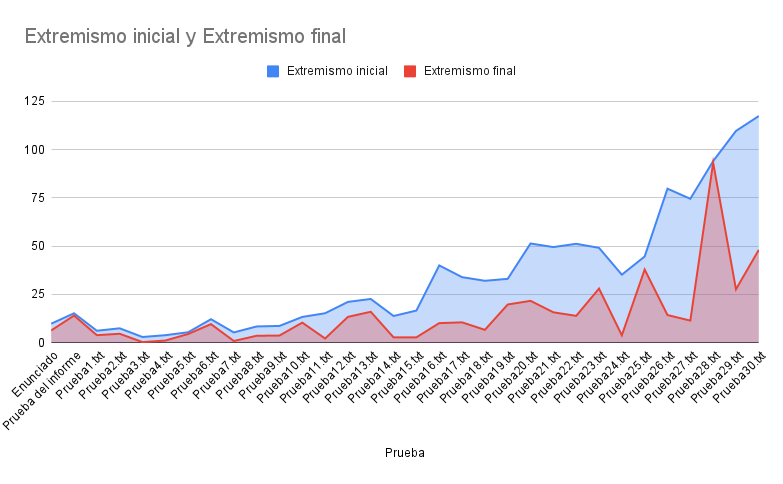
\includegraphics[width=0.8\textwidth]{resources/extremismoiyf.png}
    \caption{Comparación entre los niveles de extremismo inicial y final obtenidos en las pruebas}
\end{figure}

\subsubsection*{Grafica de Costo total y Extremismo final}
La siguiente gráfica permite observar que, en general, a medida que aumenta el costo total disponible, el extremismo final tiende a disminuir. Esto indica que el modelo es capaz de reducir la polarización cuando se le otorgan más recursos para realizar movimientos. 

\begin{figure}[H]
    \centering
    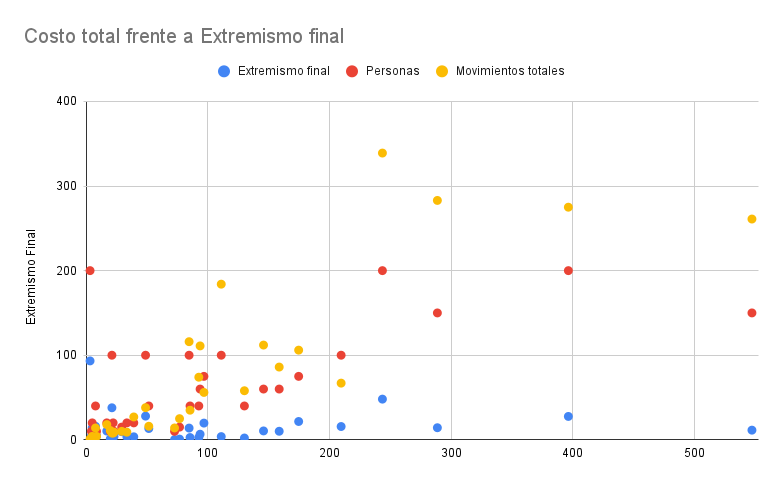
\includegraphics[width=0.8\textwidth]{resources/costototalvsextremismofinal.png}
    \caption{Comparación entre el costo total y el extremismo final obtenidos en las pruebas}
\end{figure}

\subsection{Gráfica de Costo máximo y Costo total}

A través de la siguiente gráfica se puede evidenciar que en la mayoría de casos el costo total obtenido por el modelo se mantiene significativamente por debajo del costo inicial, lo que sugiere que el modelo no requiere agotar completamente el costo disponible para alcanzar soluciones óptimas.

\begin{figure}[H]
    \centering
    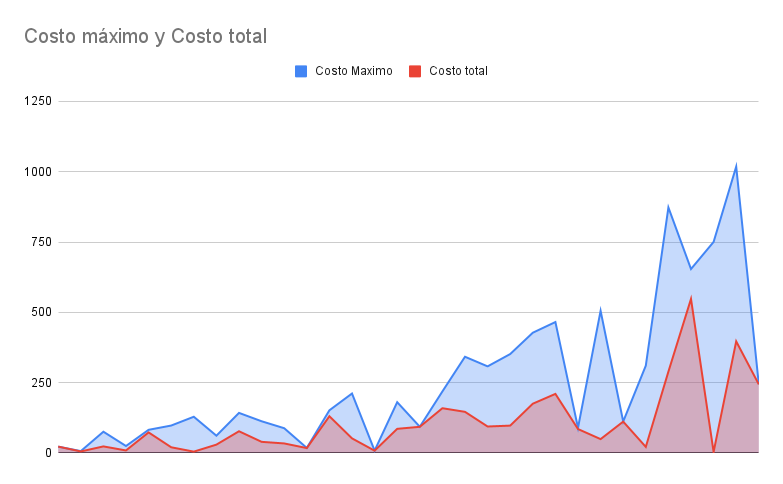
\includegraphics[width=0.8\textwidth]{resources/costomaximoycostototal.png}
    \caption{Comparación entre el costo máximo asignado y el costo total obtenido por el modelo}
\end{figure}


\subsubsection*{Gráfica de Movimientos máximos permitidos y Movimientos totales}
La siguiente gráfica evidencia  que en la mayoría de los casos, se observa que los movimientos totales tienden a ser iguales o ligeramente inferiores al máximo permitido, lo que indica que el modelo aprovecha casi todo el margen de acción disponible para cumplir su objetivo. Sin embargo, en algunas instancias los movimientos totales son considerablemente menores, lo cual puede deberse a restricciones impuestas por el costo total permitido o a configuraciones en las que no es necesario agotar el máximo de movimientos para minimizar el extremismo. 

\begin{figure}[H]
    \centering
    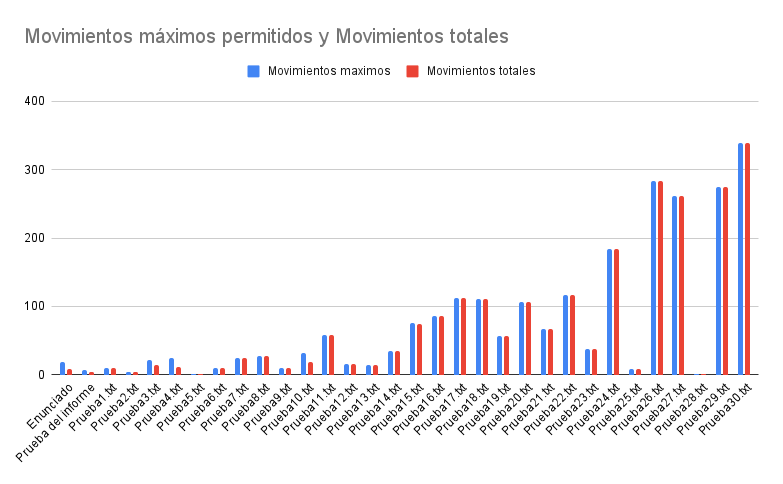
\includegraphics[width=0.8\textwidth]{resources/movimientosmaximosytotales.png}
    \caption{Comparación entre los movimientos máximos permitidos y los totales realizados por el modelo}
\end{figure}

\section{Conclusiones}

A partir del desarrollo e implementación del modelo para minimizar el extremismo presente en una población (MinExt), se pueden destacar diversas conclusiones importantes:

\begin{itemize}
    \item El modelo desarrollado permite reducir eficazmente el nivel total de extremismo en una población, siempre y cuando se disponga de suficientes recursos económicos y logísticos. Los resultados obtenidos en las pruebas muestran una reducción significativa del extremismo, especialmente en escenarios con mayor flexibilidad en términos de costo y número máximo de movimientos permitidos.

    \item La estrategia implementada mediante programación entera mixta y técnicas de optimización combinatoria (Branch and Bound) resultó adecuada para resolver el problema planteado, obteniendo soluciones óptimas o cercanas a la óptima en tiempos aceptables de ejecución.

    \item Se observó que la complejidad computacional aumenta considerablemente con el incremento del número de personas y opiniones, así como con restricciones más estrictas sobre costos y movimientos máximos. Esto implica que, en escenarios reales, es crucial balancear adecuadamente estas restricciones para mantener un equilibrio entre precisión y viabilidad del tiempo de procesamiento.

    \item La interfaz gráfica desarrollada facilita significativamente la interacción del usuario con el modelo, permitiendo una comprensión inmediata de los resultados a través de gráficos comparativos y resúmenes numéricos claros. Esto mejora la accesibilidad y utilidad del modelo para usuarios no especializados en técnicas avanzadas de optimización.

    \item Propuestas para investigaciones futuras: explorar técnicas alternativas que optimicen aún más el tiempo de solución para instancias mayores o incorporar métodos heurísticos para manejar situaciones de alta complejidad computacional.

    \item Finalmente, se destaca la importancia del hardware utilizado, ya que el rendimiento del equipo puede afectar notablemente el tiempo necesario para alcanzar soluciones factibles en problemas de mayor tamaño. Esto subraya la necesidad de disponer de infraestructura tecnológica adecuada en contextos donde se implementen modelos de optimización complejos.



\end{itemize}

\section{Referencias}

\begin{itemize}
    \item Ahuja, R. K., Magnanti, T. L., \& Orlin, J. B. (1993). \textit{Network Flows: Theory, Algorithms, and Applications}. Prentice Hall.

    \item Nemhauser, G. L., \& Wolsey, L. A. (1999). \textit{Integer and Combinatorial Optimization}. Wiley-Interscience.

    \item Rossi, F., Van Beek, P., \& Walsh, T. (2006). \textit{Handbook of Constraint Programming}. Elsevier.

    \item Flask. (s.f.). \textit{Flask Documentation}. Recuperado de: \url{https://flask.palletsprojects.com}

    \item MiniZinc. (s.f.). \textit{MiniZinc Handbook 2.5.0}. Recuperado de: \url{https://www.minizinc.org/doc-2.5.0/en/index.html}

    \item COIN-OR Branch and Cut. (s.f.). \textit{CBC User Guide}. Recuperado de: \url{https://github.com/coin-or/Cbc}

    \item Chart.js. (s.f.). \textit{Chart.js Documentation}. Recuperado de: \url{https://www.chartjs.org/docs/latest/}

    \item TailwindCSS. (s.f.). \textit{TailwindCSS Documentation}. Recuperado de: \url{https://tailwindcss.com/docs}
\end{itemize}




\end{document}
